\documentclass[mathserif, aspectratio=169]{beamer}
\usetheme{Hannover}
\usecolortheme{dolphin}
\usepackage{amsmath}
\usepackage{amssymb}
\usepackage{amsfonts}
\usepackage{hyperref}
\usepackage{graphicx}

\usepackage{lmodern}
\usepackage{beamerthemeshadow}

\beamertemplatenavigationsymbolsempty
%\beameruncovermixins{\opaqueness<1>{25}}{\opaqueness<2>{15}}

\title{local connection game}
\author{Tobias Guggenmos}

\newtheorem{Def}{Definition}
\newtheorem{Ax}{$\mathfrak{Axiom}$}
\newtheorem{Sa}{Satz}


\begin{document}
\begin{frame}
\titlepage
\end{frame}

\begin{frame}
\tableofcontents
\end{frame}

\section{Einf\"uhrung in die Graphentheorie}

\begin{frame}
\begin{Def}
Ein \textbf{Graph} ist eine abstrakte Struktur die eine Menge von Objekten (\textbf{Knoten}) zusammen mit den zwischen diesen Objekten bestehenden paarweisen Verbindungen (\textbf{Kanten}) repr\"asentiert. Kanten k\"onnen \textbf{gerichtet} oder \textbf{ungerichtet} sein.
\end{Def}
\begin{tabbing}
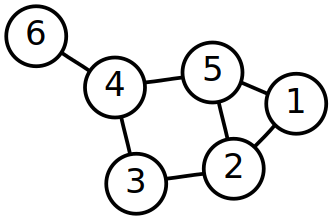
\includegraphics[height=4cm]{pics/6n-graf.png}
\=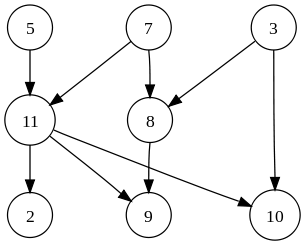
\includegraphics[height=4cm]{pics/directed-graph.png}\\
Ungerichteter Graph\>Gerichteter Graph
\end{tabbing}
\end{frame}

\section{Simulation des Internets durch Graphentheorie}
\begin{frame}
Zum besseren Verst\"andnis der (In)Effektivit\"at von Computernetzwerken, versucht man diese mithilfe der Graphentheorie zu untersuchen.
\begin{tabbing}
\hspace{5cm}\=\\
Verbundene Rechner \>$\longrightarrow$Knoten\\
Verbindungen\>$\longrightarrow$Kanten\\\\
Einfaches Beispiel:\>simple network formation game of\\\> Fabrikant et al.(2003) \\\>(local connection game)
\end{tabbing}
\end{frame}
\begin{frame}
\begin{block}
{Local Connection Game}
\begin{itemize}
        \item Der Netzwerkgraph ist ungerichtet
        \item Jeder Knoten hat Kosten
        \item Jeder Knoten handelt eigenn\"utzig, versucht also seine eigenen Kosten zu reduzieren.
        \item Jeder Knoten kann Kanten (Verbindungen) kaufen, die dann jeder nutzen kann, eine Kante kostet $\alpha$
        \item Mit der Distanz zweier Knoten $dist(a,b)$ bezeichnet man die Anzahl der (existierenden) Kanten, die f\"ur eine Verbindung ben\"otigt werden, ist eine Verbindung nicht m\"oglich, ist die Distanz $\infty$
        \item Jeder Knoten bezahlt f\"ur alle selbst gekauften Kanten $+$ die jeweiligen Distanzen zu allen anderen Knoten
        \item Mit den sozialen Kosten bezeichnet man die Summe der Kosten aller Knoten. Sie sind ein Richtwert f\"ur die Effzienz des Netzwerks.
\end{itemize}
\end{block}
\end{frame}

\begin{frame}
\begin{block}
{In Formeln}
Kosten eines Knotens u:
\[k(u)=\alpha n_u + {\sum}_v dist(u,v)\]
Soziale Kosten:
\[{\sum}_u k(u)= \alpha n + {\sum}_{u\not=v} dist (u,v)\]
\end{block}
\end{frame}
\section{Erkentnisse}
\begin{frame}
{Optimale L\"osungen}
%\begin{block}{Optimale L\"osungen}
\begin{columns}
\column{.5\textwidth}
\textbf{$\alpha \leq 1$}\\
Vollst\"andiger Graph\\
Nash Gleichgewicht\\
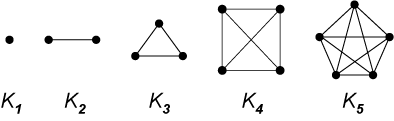
\includegraphics[width=5cm]{pics/Complete_graph_example.png}
\column{.5\textwidth}
\textbf{$\alpha \geq 2$}\\
Stern\\
Nash Gleichgewicht f\"ur $\alpha \geq 1$ \\
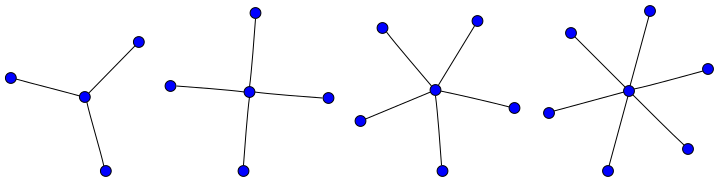
\includegraphics[width=5cm]{pics/star.png}
\end{columns}
\begin{exampleblock}
{Nash Gleichgewicht}
Kein Knoten hat einen Anlass, am Graphen etwas \"andern, da es ihm keinerlei Vorteil bringt.
\end{exampleblock}

%\end{block}
\end{frame}


\end{document}
